\chapter{How does SmartResolution work?}\label{appendix:workflow}

Online Dispute Resolution is aimed at lawyers (hereafter known as Agents), representing their clients through the ODR platform. Optionally, we have mediators, whose aim is to intervene as an independent third-party if the two opposing lawyers are struggling to reach a resolution. SmartResolution supports both of these roles.

\section{Roles in the system}

\begin{figure}[ht!]
  \centering
    \ifimages
    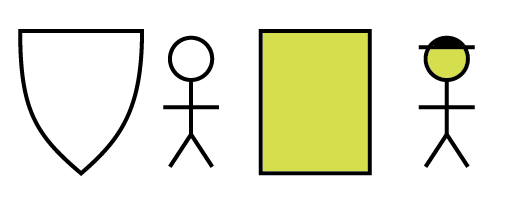
\includegraphics[width=0.7\textwidth]{workflow/roles}
    \fi
    \caption{Roles in the system}
  \label{workflow:roles}
\end{figure}

In figure~\ref{workflow:roles}, from left to right, we have:

\begin{itemize}
\item Law Firm - an Organisation account.
\item Agent - an Individual account, belonging to a Law Firm.
\item Mediation Centre - an Organisation account.
\item Mediator - an Individual account, belonging to a Mediation Centre.
\end{itemize}

\section{Setting up}

Before a dispute can be opened on SmartResolution, both Agents must be registered to the system. For each Agent to be registered, their Law Firm must also be registered.

\begin{enumerate}
\item Law Firm A registers an account and logs in.
\item Law Firm A creates an account for Agent A.
\item Law Firm B registers an account and logs in.
\item Law Firm B creates an account for Agent B.
\end{enumerate}

\section{Creating a dispute}

\subsection{Assigning the dispute to the relevant parties}

\begin{figure}[ht!]
  \centering
    \ifimages
    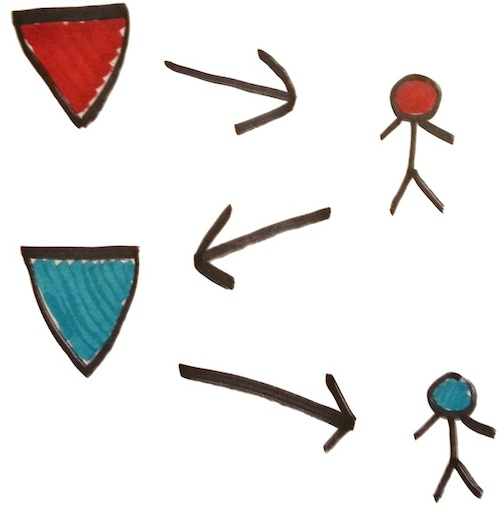
\includegraphics[width=0.5\textwidth]{workflow/dispute_creation}
    \fi
    \caption{Creating a dispute}
  \label{workflow:disputeCreation}
\end{figure}

Figure~\ref{workflow:disputeCreation} demonstrates:

\begin{itemize}
\item Law Firm A creates a dispute, assigning it to Agent A.
\item Agent A fills in their summary for the dispute and opens the dispute against Law Firm B.
\item Law Firm B assigns the dispute to Agent B.
\item Agent B fills in their summary to accept the dispute.
\end{itemize}

\subsection{Negotiating a lifespan}

\begin{figure}[ht!]
  \centering
    \ifimages
    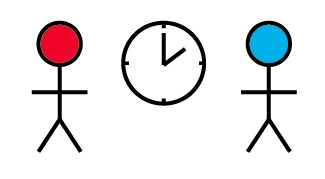
\includegraphics[width=0.6\textwidth]{workflow/lifespan}
    \fi
    \caption{Negotiating a lifespan}
  \label{workflow:lifespan}
\end{figure}

The agents need to agree on a start and end time for the dispute. A dispute can last for hours, weeks or months, depending on the preferences of the agents involved.

A lifespan can be re-negotiated at any point in the dispute process.

\subsection{The dispute begins}

\begin{figure}[ht!]
  \centering
    \ifimages
    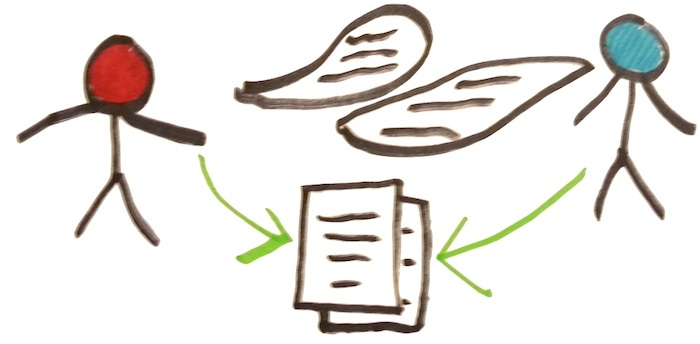
\includegraphics[width=0.6\textwidth]{workflow/dispute}
    \fi
    \caption{The dispute begins}
  \label{workflow:dispute}
\end{figure}

With a lifespan negotiated and a dispute fully assigned, the agents are now able to communicate through the SmartResolution chat facility and upload documents as evidence.

\section{Mediation}

Sometimes, disputes may not be solved without the aid of an independent mediator. SmartResolution supports Mediation Centres and Mediators: at any point in an active dispute, either agent can propose mediation.

\begin{figure}[ht!]
  \centering
    \ifimages
    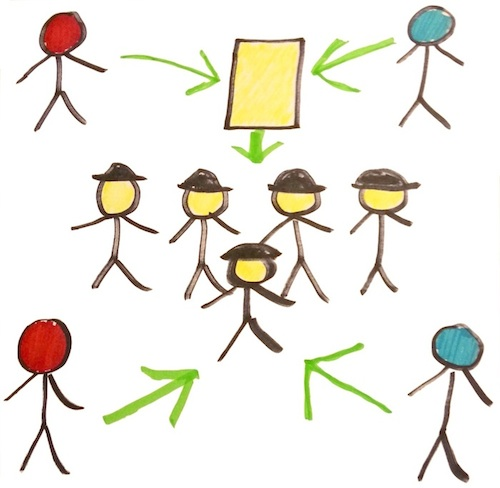
\includegraphics[width=0.5\textwidth]{workflow/mediation_creation}
    \fi
    \caption{Mediation}
  \label{workflow:mediation}
\end{figure}

\begin{itemize}
\item An agent proposes to use Mediation Centre `MC' to mediate the dispute.
\item The other agent accepts. `MC' is notified that they are now the Mediation Centre of the dispute.
\item `MC' provides a list of all available Mediators.
\item The agents are free to peruse the profiles of the Mediators, reading their CVs and contacting them externally if necessary.
\item An agent proposes to use Mediator M to mediate the dispute.
\item The other agent agrees. The dispute is now in mediation.
\end{itemize}

\begin{figure}[ht!]
  \centering
    \ifimages
    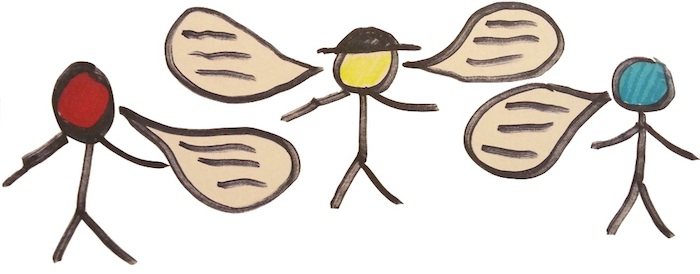
\includegraphics[width=0.6\textwidth]{workflow/mediation}
    \fi
    \caption{Mediation in action}
  \label{workflow:mediationAction}
\end{figure}

With the dispute in mediation, all communication is done through the mediator, unless the mediator proposes ``Round-Table Communication" and both agents accept. In this case, a three-person chat is unlocked. At any time, either agent can revoke Round-Table Communication.

\section{Modules}

If there is a relevant SmartResolution Module installed to the system, that may help the Agents to reach a resolution.

For example, let's say we have a `Maritime Collision' module. This adds a 'Maritime Collision' dispute type to the dispute-creation screen.

With the dispute type set to `Maritime Collision', an additional option is unlocked: Agents are able to let the module ask them structured, maritime-law-specific questions. The module then interprets their answers according to the law, and automatically suggests a resolution.

Modules can help to cut out mediators altogether, if they act as `mediator AI' - saving everyone valuable time and money. This is what sets SmartResolution apart from the competition.